\documentclass[a4paper, 14pt]{extarticle}

% Поля
%--------------------------------------
\usepackage{geometry}
\geometry{a4paper,tmargin=2cm,bmargin=2cm,lmargin=3cm,rmargin=1cm}
%--------------------------------------


%Russian-specific packages
%--------------------------------------
\usepackage[T2A]{fontenc}
\usepackage[utf8]{inputenc}
\usepackage[english, main=russian]{babel}
%--------------------------------------

\usepackage{textcomp}

% Красная строка
%--------------------------------------
\usepackage{indentfirst}
%--------------------------------------


%Graphics
%--------------------------------------
\usepackage{graphicx}
\graphicspath{ {./images/} }
\usepackage{wrapfig}
%--------------------------------------

% Полуторный интервал
%--------------------------------------
\linespread{1.3}
%--------------------------------------

%Выравнивание и переносы
%--------------------------------------
% Избавляемся от переполнений
\sloppy
% Запрещаем разрыв страницы после первой строки абзаца
\clubpenalty=10000
% Запрещаем разрыв страницы после последней строки абзаца
\widowpenalty=10000
%--------------------------------------

%Списки
\usepackage{enumitem}

%Подписи
\usepackage{caption}

%Гиперссылки
\usepackage{hyperref}

\hypersetup {
	unicode=true
}

%Рисунки
%--------------------------------------
\DeclareCaptionLabelSeparator*{emdash}{~--- }
\captionsetup[figure]{labelsep=emdash,font=onehalfspacing,position=bottom}
%--------------------------------------

\usepackage{tempora}

%Листинги
%--------------------------------------
\usepackage{listings}
\lstset{
  basicstyle=\ttfamily\footnotesize,
  %basicstyle=\footnotesize\AnkaCoder,        % the size of the fonts that are used for the code
  breakatwhitespace=false,         % sets if automatic breaks shoulbd only happen at whitespace
  breaklines=true,                 % sets automatic line breaking
  captionpos=t,                    % sets the caption-position to bottom
  inputencoding=utf8,
  frame=single,                    % adds a frame around the code
  keepspaces=true,                 % keeps spaces in text, useful for keeping indentation of code (possibly needs columns=flexible)
  keywordstyle=\bf,       % keyword style
  numbers=left,                    % where to put the line-numbers; possible values are (none, left, right)
  numbersep=5pt,                   % how far the line-numbers are from the code
  xleftmargin=25pt,
  xrightmargin=25pt,
  showspaces=false,                % show spaces everywhere adding particular underscores; it overrides 'showstringspaces'
  showstringspaces=false,          % underline spaces within strings only
  showtabs=false,                  % show tabs within strings adding particular underscores
  stepnumber=1,                    % the step between two line-numbers. If it's 1, each line will be numbered
  tabsize=2,                       % sets default tabsize to 8 spaces
  title=\lstname                   % show the filename of files included with \lstinputlisting; also try caption instead of title
}
%--------------------------------------

%%% Математические пакеты %%%
%--------------------------------------
\usepackage{amsthm,amsfonts,amsmath,amssymb,amscd}  % Математические дополнения от AMS
\usepackage{mathtools}                              % Добавляет окружение multlined
\usepackage[perpage]{footmisc}
%--------------------------------------

%--------------------------------------
%			НАЧАЛО ДОКУМЕНТА
%--------------------------------------

\begin{document}

%--------------------------------------
%			ТИТУЛЬНЫЙ ЛИСТ
%--------------------------------------
\begin{titlepage}
\thispagestyle{empty}
\newpage


%Шапка титульного листа
%--------------------------------------
\vspace*{-60pt}
\hspace{-65pt}
\begin{minipage}{0.3\textwidth}
\hspace*{-20pt}\centering

\includegraphics[width=\textwidth]{emblem}
\end{minipage}
\begin{minipage}{0.67\textwidth}\small \textbf{
\vspace*{-0.7ex}
\hspace*{-6pt}\centerline{Министерство науки и высшего образования Российской Федерации}
\vspace*{-0.7ex}
\centerline{Федеральное государственное бюджетное образовательное учреждение }
\vspace*{-0.7ex}
\centerline{высшего образования}
\vspace*{-0.7ex}
\centerline{<<Московский государственный технический университет}
\vspace*{-0.7ex}
\centerline{имени Н.Э. Баумана}
\vspace*{-0.7ex}
\centerline{(национальный исследовательский университет)>>}
\vspace*{-0.7ex}
\centerline{(МГТУ им. Н.Э. Баумана)}}
\end{minipage}
%--------------------------------------

%Полосы
%--------------------------------------
\vspace{-25pt}
\hspace{-35pt}\rule{\textwidth}{2.3pt}

\vspace*{-20.3pt}
\hspace{-35pt}\rule{\textwidth}{0.4pt}
%--------------------------------------

\vspace{1.5ex}
\hspace{-35pt} \noindent \small ФАКУЛЬТЕТ\hspace{80pt} <<Информатика и системы управления>>

\vspace*{-16pt}
\hspace{47pt}\rule{0.83\textwidth}{0.4pt}

\vspace{0.5ex}
\hspace{-35pt} \noindent \small КАФЕДРА\hspace{50pt} <<Теоретическая информатика и компьютерные технологии>>

\vspace*{-16pt}
\hspace{30pt}\rule{0.866\textwidth}{0.4pt}

\vspace{11em}

\begin{center}
\Large {\bf Контрольная работа № 2.2} \\
\large {\bf по курсу <<Разработка мобильных приложений>>} \\
\large <<HTTP JSON parser>>
\end{center}\normalsize

\vspace{8em}


\begin{flushright}
  {Студентка группы ИУ9-72Б Самохвалова П. С. \hspace*{15pt}\\
  \vspace{2ex}
  Преподаватель Посевин Д. П.\hspace*{15pt}}
\end{flushright}

\bigskip

\vfill


\begin{center}
\textsl{Москва 2023}
\end{center}
\end{titlepage}
%--------------------------------------
%		КОНЕЦ ТИТУЛЬНОГО ЛИСТА
%--------------------------------------

\renewcommand{\ttdefault}{pcr}

\setlength{\tabcolsep}{3pt}
\newpage
\setcounter{page}{2}

\section{Задание}\label{Sect::task}

Реализовать мобильное приложение выполняющее разбор данных в формате JSON получаемых по протоколу HTTP.

Индивидуальный вариант:

\verb|https://mysafeinfo.com/api/data?list=jquery&format=json|

\section{Практическая реализация}\label{Sect::code}

Исходный код программы представлен в листинге~\ref{lst:code1}.

\begin{lstlisting}[language={},caption={},label={lst:code1}]
package com.example.httpjson

import android.os.Build
import android.os.Bundle
import android.os.StrictMode
import android.os.StrictMode.ThreadPolicy
import android.widget.ListView
import android.widget.Toast
import androidx.appcompat.app.AppCompatActivity
import org.json.JSONArray
import java.net.HttpURLConnection
import java.net.URL


class MainActivity : AppCompatActivity() {


    override fun onCreate(savedInstanceState: Bundle?) {
        super.onCreate(savedInstanceState)
        setContentView(R.layout.activity_main)

        if (Build.VERSION.SDK_INT > 9) {
            val policy = ThreadPolicy.Builder().permitAll().build()
            StrictMode.setThreadPolicy(policy)
        }

        val url = "https://mysafeinfo.com/api/data?list=jquery&format=json"
        val connection = URL(url).openConnection() as HttpURLConnection
        val responseCode = connection.responseCode

        try {
            val data = connection.inputStream.bufferedReader().use { it.readText() }
            // ... do something with "data"
            val toast = Toast.makeText(applicationContext, data, Toast.LENGTH_LONG)
            toast.show()
            hanldeJson(data)

        } finally {
            connection.disconnect()
        }

    }




    private fun hanldeJson(jsonString: String?) {

        val jsonArray = JSONArray(jsonString)

        val list = ArrayList<Jquery>()
        var x = 0
        while (x < jsonArray.length()) {

            val jsonObject = jsonArray.getJSONObject(x)

            list.add(
                Jquery(
                    jsonObject.getDouble("Version"),
                    jsonObject.getString("ReleaseDate") ,
                    jsonObject.getString("LatestUpdate") ,
                    jsonObject.getString("Size") ,
                    jsonObject.getString("Notes") ,
                    jsonObject.getInt("ID"),
            ))

            x++
        }

        val adapter = ListAdapte(this, list)
        val list2: ListView = findViewById(R.id.jquery_list);
        list2.setAdapter(adapter);

        val toast = Toast.makeText(applicationContext, x.toString(), Toast.LENGTH_LONG)


        toast.show()


    }
}


package com.example.httpjson

data class Jquery (val version: Double, val releaseDate: String, val latestUpdate: String, val size: String, val notes: String, val id: Int ) {

}


package com.example.httpjson

import android.annotation.SuppressLint
import android.content.Context
import android.view.LayoutInflater
import android.view.View
import android.view.ViewGroup
import android.widget.BaseAdapter
import android.widget.Toast
import androidx.appcompat.widget.AppCompatTextView

class ListAdapte (val context: Context, val list: ArrayList<Jquery>) : BaseAdapter() {
    override fun getCount(): Int {
        return list.size
    }

    override fun getItem(position: Int): Any {
        return list[position]
    }

    override fun getItemId(position: Int): Long {
        return position.toLong()
    }

    @SuppressLint("MissingInflatedId", "ViewHolder")
    override fun getView(position: Int, countertView: View?, parent: ViewGroup?): View {

        val view: View = LayoutInflater.from(context).inflate(R.layout.row_layout,parent,false)
        val jqueryVersion = view.findViewById(R.id.jquery_version) as AppCompatTextView
        val jqueryReleaseDate = view.findViewById(R.id.jquery_releaseDate) as AppCompatTextView
        val jqueryLatestUpdate = view.findViewById(R.id.jquery_latestUpdate) as AppCompatTextView
        val jquerySize = view.findViewById(R.id.jquery_size) as AppCompatTextView
        val jqueryNotes = view.findViewById(R.id.jquery_notes) as AppCompatTextView
        val jqueryId = view.findViewById(R.id.jquery_id) as AppCompatTextView

        jqueryVersion.text = list[position].version.toString()
        jqueryReleaseDate.text = list[position].releaseDate
        jqueryLatestUpdate.text = list[position].latestUpdate
        jquerySize.text = list[position].size
        jqueryNotes.text = list[position].notes
        jqueryId.text = list[position].id.toString()

        view.setOnClickListener({
            Toast.makeText(context, "Version: ${jqueryVersion.text}\nReleaseDate: ${jqueryReleaseDate.text}\nLatestUpdate: ${jqueryLatestUpdate.text}\nSize: ${jquerySize.text}\nNotes: ${jqueryNotes.text}\nId: ${jqueryId.text}" , Toast.LENGTH_SHORT).show()
        })

        return view
    }
}


<?xml version="1.0" encoding="utf-8"?>
<androidx.constraintlayout.widget.ConstraintLayout xmlns:android="http://schemas.android.com/apk/res/android"
    xmlns:app="http://schemas.android.com/apk/res-auto"
    xmlns:tools="http://schemas.android.com/tools"
    android:layout_width="match_parent"
    android:layout_height="match_parent"
    tools:context=".MainActivity">

    <ListView
        android:id="@+id/jquery_list"
        android:layout_width="match_parent"
        android:layout_height="match_parent"/>

</androidx.constraintlayout.widget.ConstraintLayout>



<?xml version="1.0" encoding="utf-8"?>
<LinearLayout xmlns:android="http://schemas.android.com/apk/res/android"
    android:orientation="vertical"
    android:layout_width="match_parent"
    android:layout_height="match_parent"
    android:padding="10dp">

<androidx.appcompat.widget.AppCompatTextView
    android:id="@+id/jquery_version"
    android:layout_width="match_parent"
    android:layout_height="match_parent"
    android:textSize="20sp"/>

<androidx.appcompat.widget.AppCompatTextView
    android:id="@+id/jquery_releaseDate"
    android:layout_width="match_parent"
    android:layout_height="match_parent"
    android:textSize="26sp"/>

<androidx.appcompat.widget.AppCompatTextView
    android:id="@+id/jquery_latestUpdate"
    android:layout_width="match_parent"
    android:layout_height="match_parent"
    android:textSize="16sp"/>

<androidx.appcompat.widget.AppCompatTextView
    android:id="@+id/jquery_size"
    android:layout_width="match_parent"
    android:layout_height="match_parent"
    android:textSize="16sp"/>

<androidx.appcompat.widget.AppCompatTextView
    android:id="@+id/jquery_notes"
    android:layout_width="match_parent"
    android:layout_height="match_parent"
    android:textSize="16sp"/>

<androidx.appcompat.widget.AppCompatTextView
    android:id="@+id/jquery_id"
    android:layout_width="match_parent"
    android:layout_height="match_parent"
    android:textSize="16sp"/>

</LinearLayout>



\end{lstlisting}

\section{Результаты}\label{Sect::res}

Результаты работы программы представлены на рисунках~\ref{fig:img1}~--~\ref{fig:img3}.    

\begin{figure}[!htb]
	\centering
	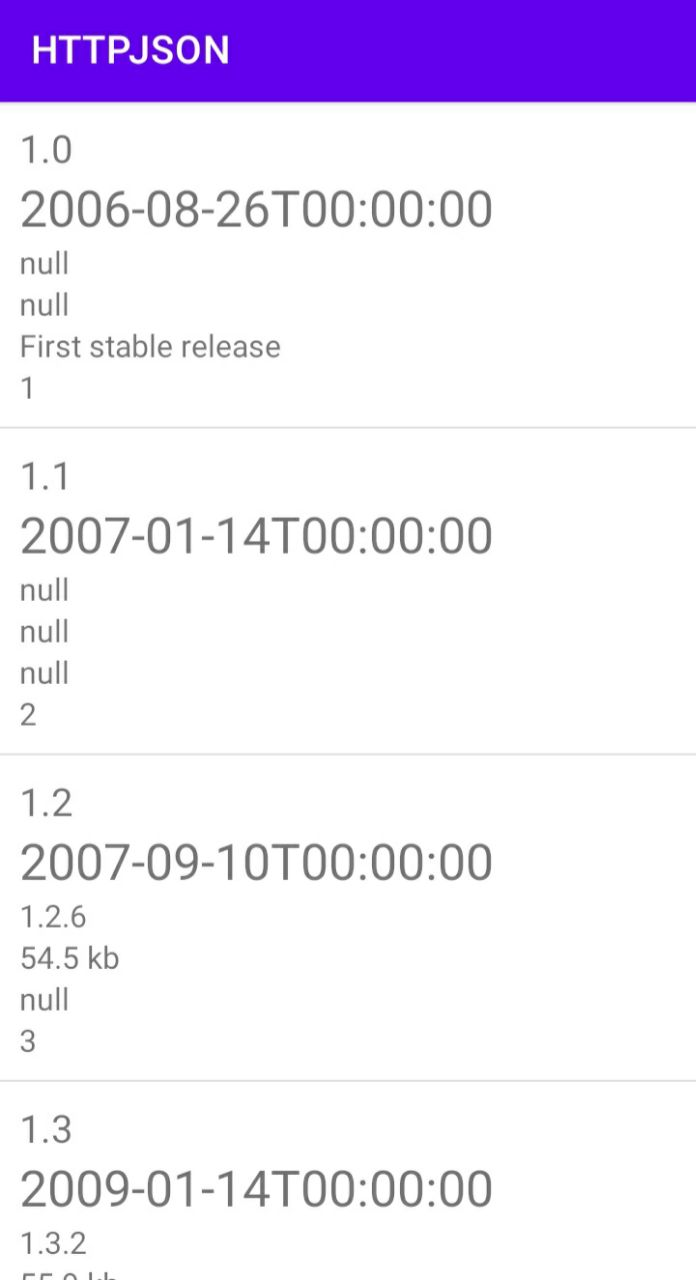
\includegraphics[width=0.8\textwidth]{img1}
\caption{Результаты}
\label{fig:img1}
\end{figure}

\begin{figure}[!htb]
	\centering
	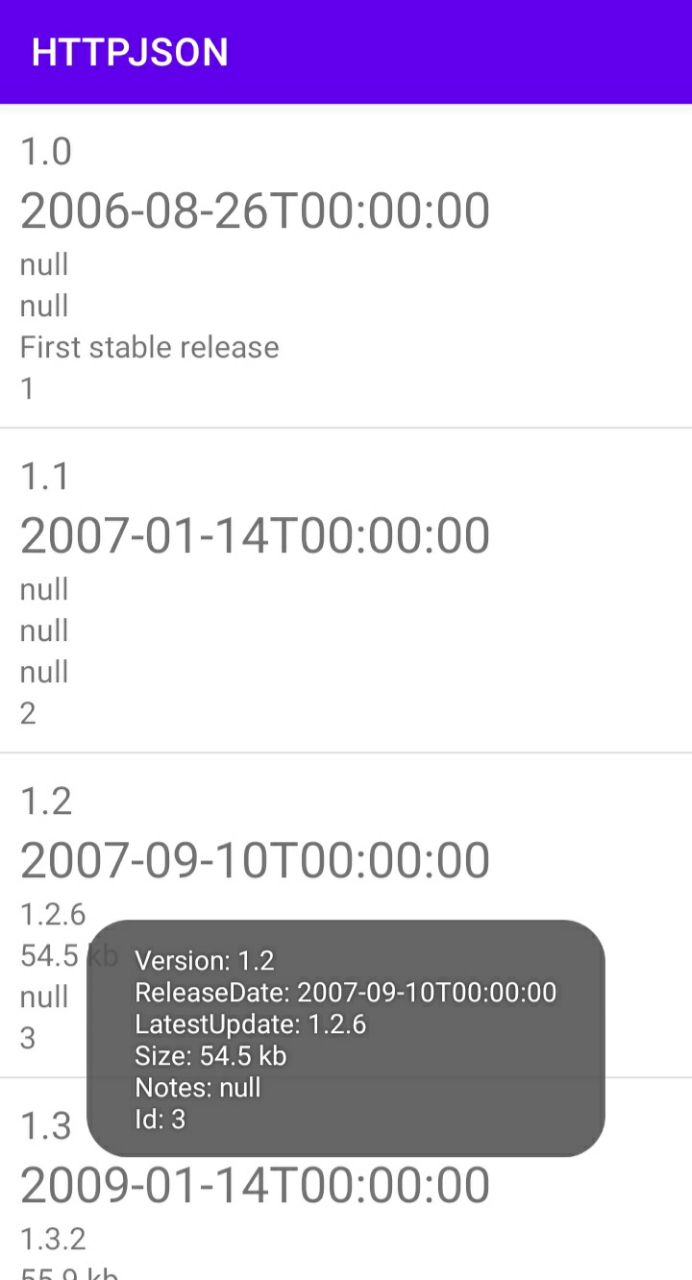
\includegraphics[width=0.8\textwidth]{img2}
\caption{Результаты}
\label{fig:img2}
\end{figure}

\begin{figure}[!htb]
	\centering
	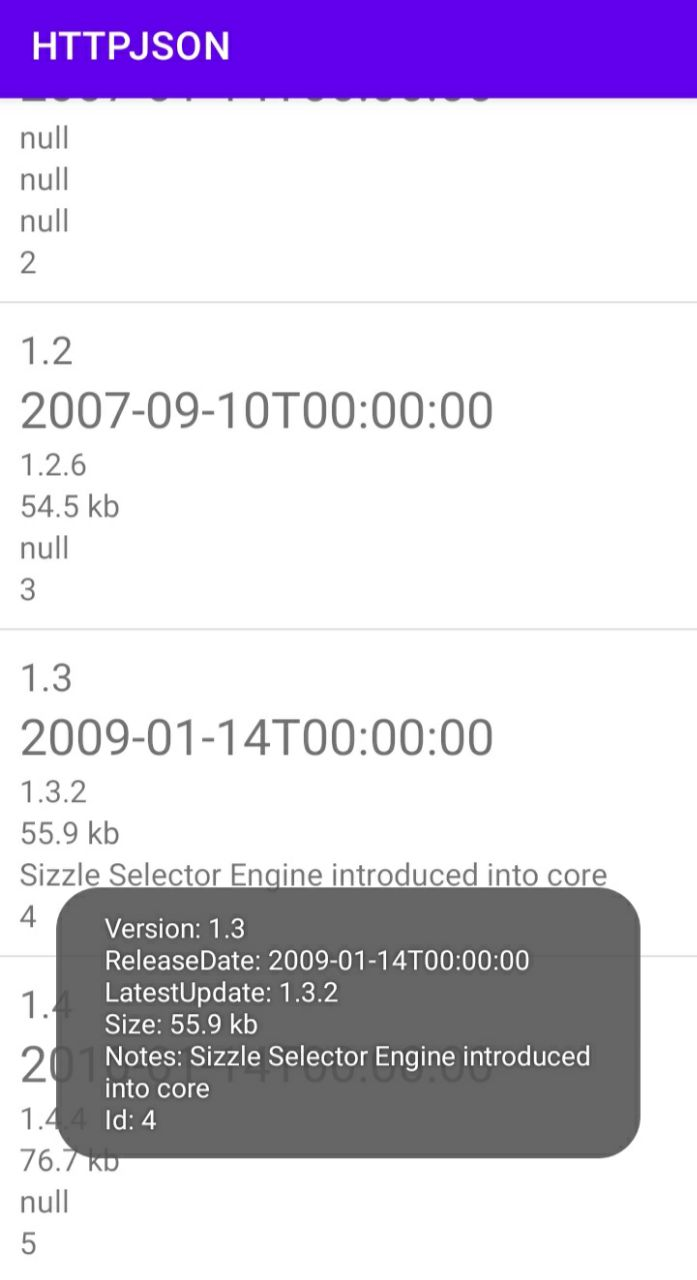
\includegraphics[width=0.8\textwidth]{img3}
\caption{Результаты}
\label{fig:img3}
\end{figure}

\section{Выводы}\label{Sect::conclusion}

В результате выполнения рубежного контроля было реализовано мобильное приложение выполняющее разбор данных в формате JSON получаемых по протоколу HTTP.

\end{document}
